\documentclass{beamer}

\usepackage[frenchb]{babel}
\usepackage[utf8]{inputenc}


\usetheme{Frankfurt}

\addtobeamertemplate{navigation symbols}{\usebeamerfont{footline}%
	\usebeamercolor[fg]{footline}
	\hspace{1em}
	\insertframenumber/\inserttotalframenumber}

\title[Outil de gestion de parcours-patient]{Outil de gestion de parcours-patient dans un hôpital de jour}
\subtitle{Soutenance de Projet R\&D}
\author{Romain ROUSSEAU}
\date{\today}


\begin{document}
	
\begin{frame}[plain]
	\titlepage
\end{frame}

\AtBeginSection[]
{
\begin{frame}
	
	\tableofcontents[currentsection, hideallsubsections]
	
\end{frame} 
}

\begin{frame}[plain]
\frametitle{Introduction}

Projet Recherche \& Développement sur l'amélioration d'un outil de gestion de parcours-patient pour l'AP-HP (Assistance publique - Hôpitaux de Paris).

\begin{figure}
	
\includegraphics[scale=0.7]{images/LOGO_APHP}
\end{figure}

\end{frame}


\begin{frame}

\frametitle{Sommaire}

\tableofcontents

\end{frame}

\section[Contexte]{Contexte}

\begin{frame}
\frametitle{Contexte}

La gestion des patients dans les hôpitaux fait l'objet de nombreux débats.

\bigbreak

\begin{itemize}
	\item Temps d'attente trop longs pour les patients
	\item Problèmes liés aux ressources disponibles (salles, personnel, ...) 
	\item Problèmes budgétaires
\end{itemize}

\end{frame}

\begin{frame}
\frametitle{Contexte}

Gestion d'un ensemble de patients réalisant des activités planifiées sur une journée.

\bigbreak

Un patient suit un "\textbf{parcours de soins}" constitué d'activités.

\bigbreak

Une activité est caractérisée par une durée et un ensemble de ressources (matérielle et personnelle). Certaines peuvent avoir des \textbf{contraintes de précédence}. 

\end{frame}

\begin{frame}
\frametitle{Exemple de parcours}
	
Exemple de parcours: Diagnostic d'obésité sévère
	
\begin{figure}
	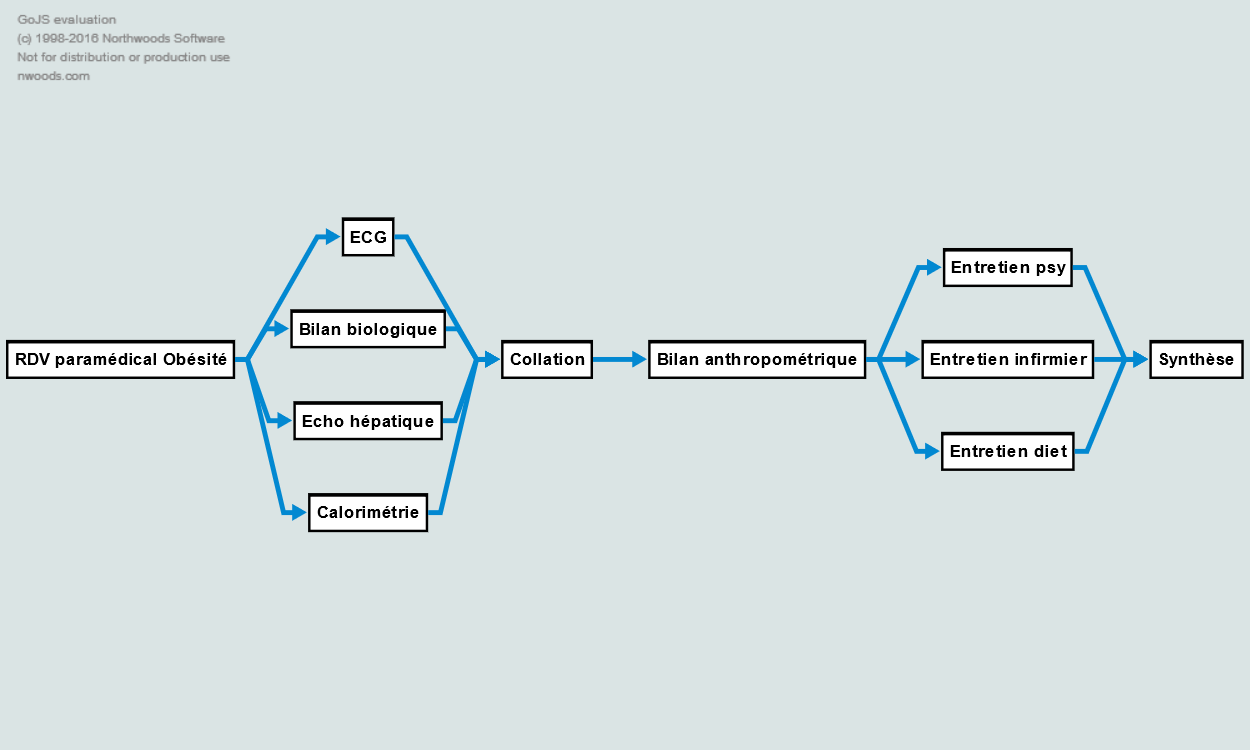
\includegraphics[scale=0.425]{images/exemple_parcours}
\end{figure}
	
\end{frame}


\begin{frame}
\frametitle{Contexte du projet}

\begin{block}{Suite de plusieurs projets consécutifs}
	\begin{description}
		\item[Projet SI et R\&D 2015-2016]: par 6 étudiants et Jean Coquelet, modélisation et développement des fonctionnalités de base
		\item[Projet R\&D 2016-2017]: par Guillaume Pochet, planification manuelle des activités
		\item[Projet R\&D 2017-2018]: par Yang Jing, ajout de fonctionnalités de gestion
	\end{description}
\end{block}

\end{frame}

\begin{frame}
\frametitle{Objectifs}

Améliorations générales de la plateforme (corrections de bugs, d'erreurs de conception, de fautes d'orthographe, etc.).

\bigbreak

Implémentation de la planification automatique des activités de soin.

\end{frame}


\section[Description]{Description du projet}
%Présentation de l'outil les pages les plus intéressantes.

\begin{frame}
\frametitle{Description du projet}

Plateforme web développée en PHP, HTML, Javascript à l'aide du framework CodeIgniter.


\begin{figure}
	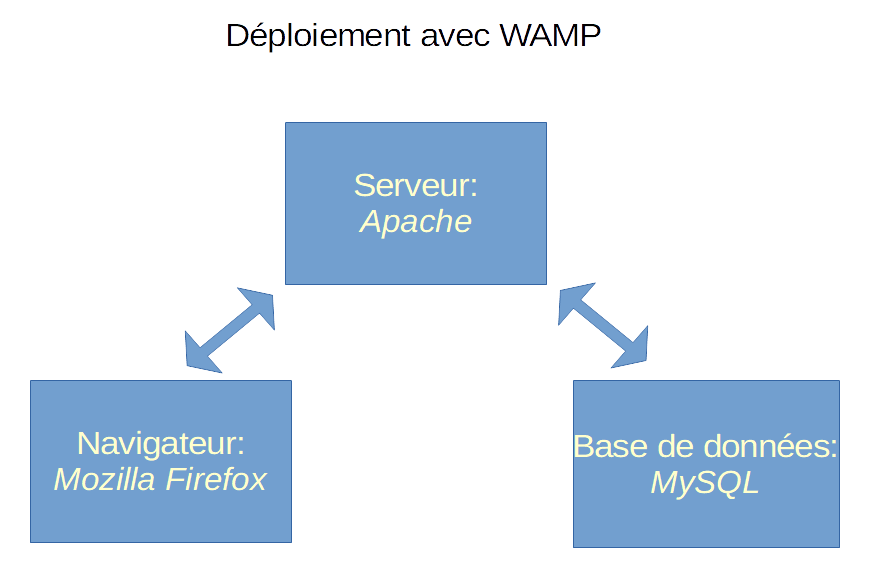
\includegraphics[scale=0.5]{images/deploiement_wamp}
\end{figure}

\end{frame}

\begin{frame}
\frametitle{Aperçu de la page d'accueil}

\begin{center}
	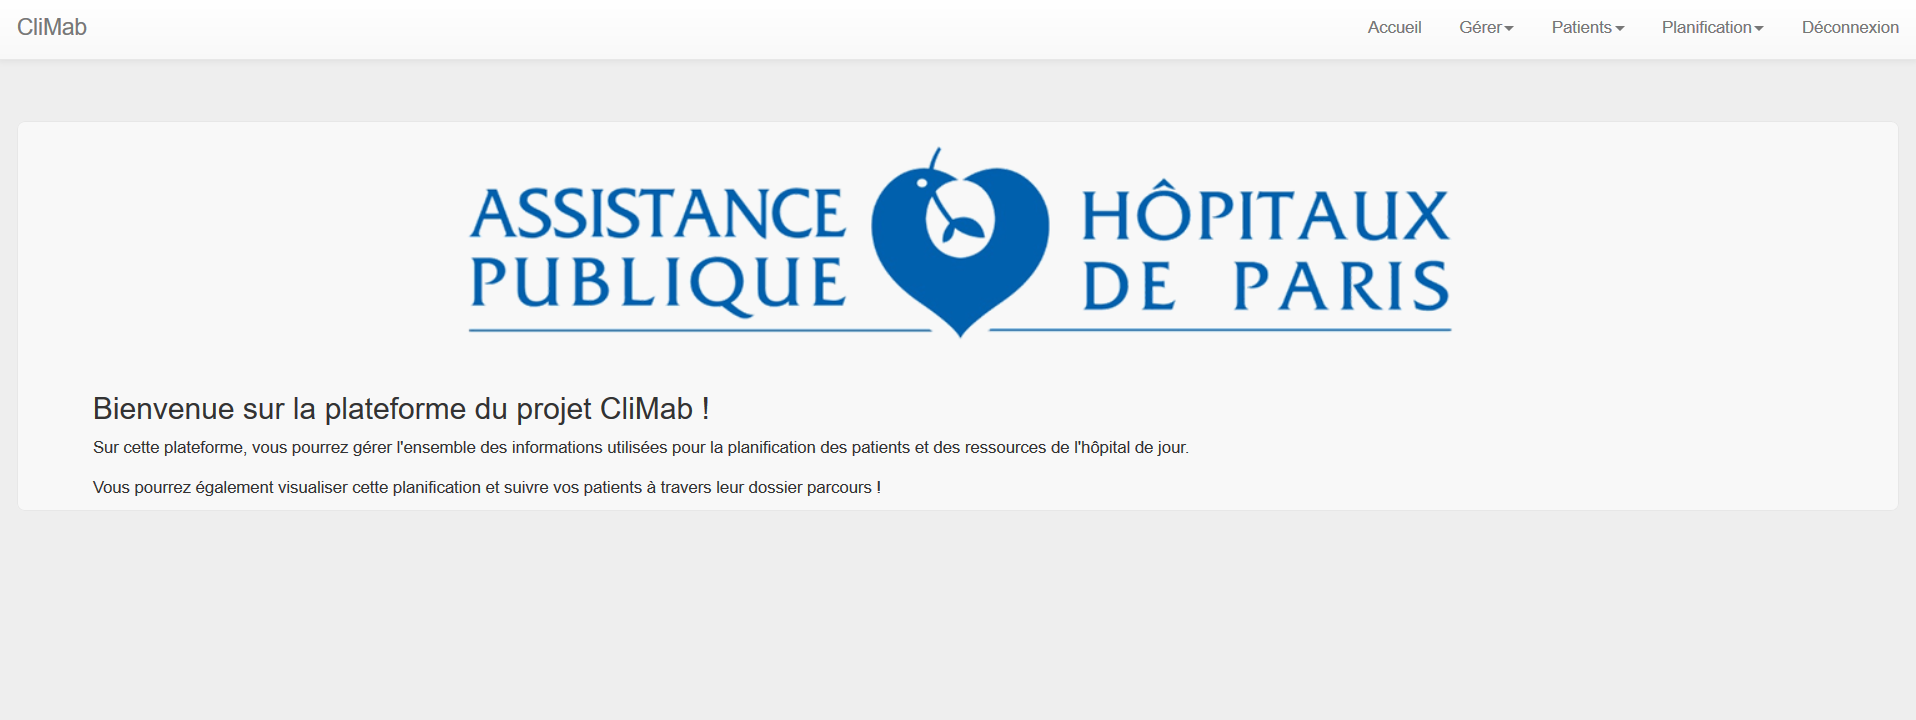
\includegraphics[scale=0.28]{images/accueil}
\end{center}

\end{frame}

\begin{frame}
\frametitle{Aperçu de la page de planification}

\begin{center}
	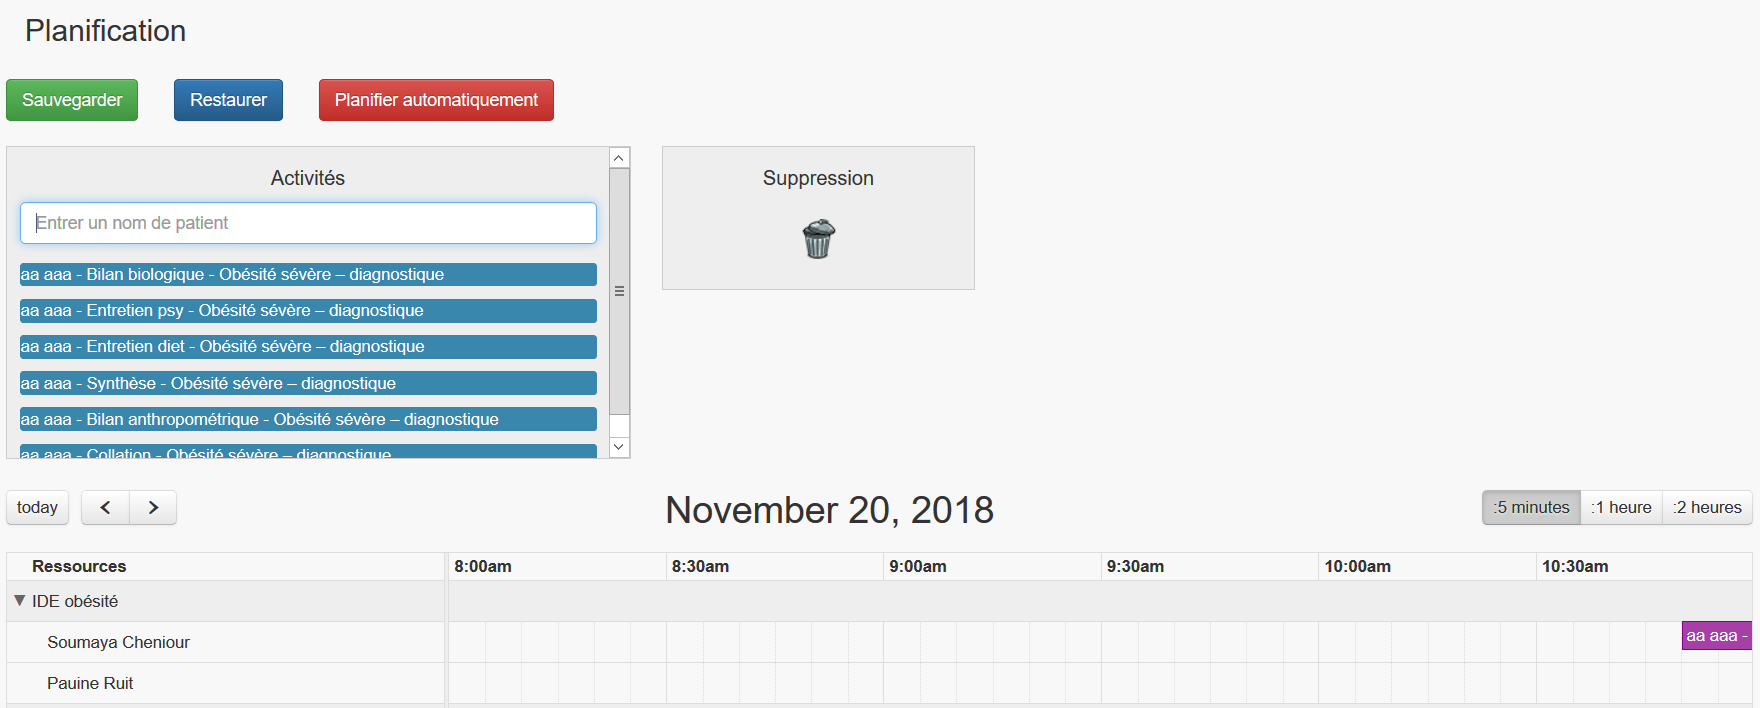
\includegraphics[scale=0.3]{images/bouton_plan_auto}
\end{center}

\end{frame}

\begin{frame}
\frametitle{Aperçu de la page de planification}

\begin{center}
	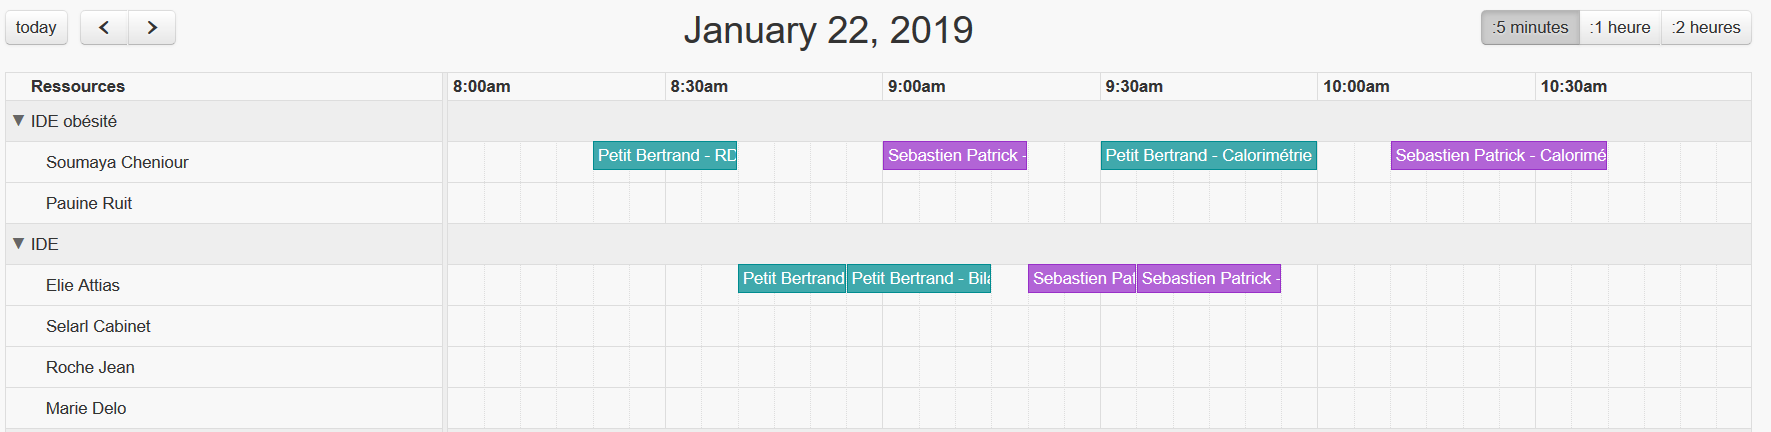
\includegraphics[scale=0.175]{images/exemple_calendrier}
\end{center}

\end{frame}


\section[Gestion de projet]{Gestion de projet}

\begin{frame}
\frametitle{Chiffrage du projet}

\begin{center}
	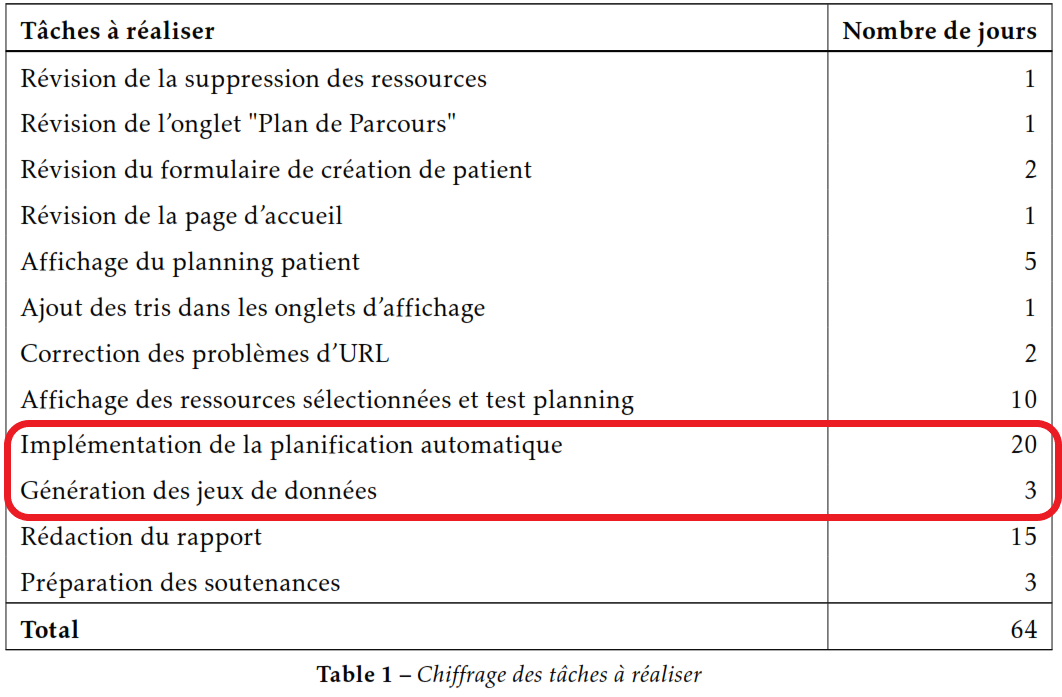
\includegraphics[scale=0.375]{images/chiffrage}
\end{center}

\end{frame}

\begin{frame}
\frametitle{Gestion de projet}

Deux livrables pour le projet:

\bigbreak

\begin{block}{Livrable à l'issue de la première partie}
	Comprend les corrections de bugs et les améliorations sur les onglets de Gestion.
\end{block}

\begin{block}{Livrable finale}
	Comprend les implémentations concernant la planification automatique.
\end{block}

\end{frame}


\section{Mise en œuvre}

\begin{frame}
\frametitle{Avant-propos sur la planification}

L'outil doit traiter des \textbf{problèmes multi-ressources} (\textit{Multi-Appointment Scheduling Problems in hospitals} en anglais).

\bigbreak

Un domaine récent de la recherche (pas avant 1995) lié aux domaines suivants: 

\begin{itemize}
	\item la prise de rendez-vous (\textit{appointment scheduling}) 
	\item le domaine de la médecine intégrée (\textit{integrated healthcare}) 
	\item les flux de patients (\textit{patient flow}) 
	\item la planification de ressources (\textit{resource scheduling}) 
	\item la gestion des infirmiers (\textit{nurse rostering})
\end{itemize}

\end{frame}

\begin{frame}
\frametitle{Avant-propos sur la planification}

Dans notre cas, 

\begin{itemize}
	\item Les patients sont planifiés jour après jour
	\item Les ressources sont le personnel, les salles et le matériel
\end{itemize}

Il est important de choisir quoi optimiser (minimiser les temps d'attente, minimiser les coûts...).

\end{frame}

\begin{frame}
\frametitle{Algorithme}

Dans un premier temps, l'objectif est de placer les activités sur le calendrier patient par patient.

\begin{center}
	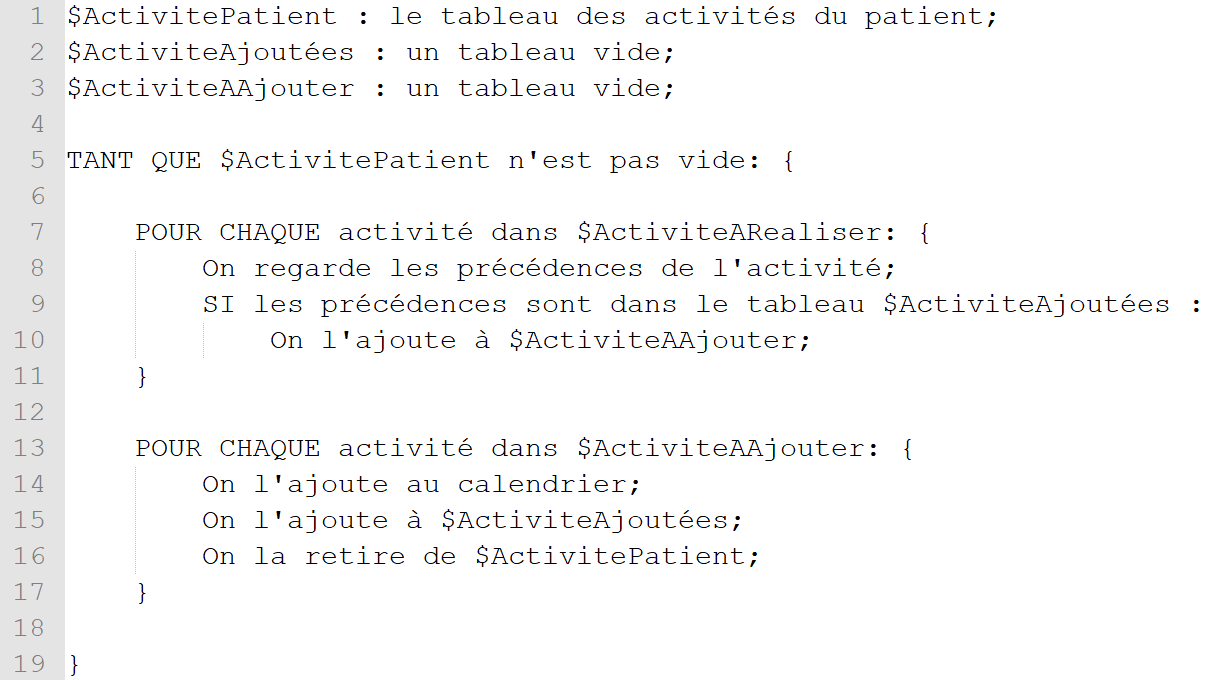
\includegraphics[scale=0.4]{images/algoPlanAuto}
\end{center}

\end{frame}

\begin{frame}

\begin{center}
	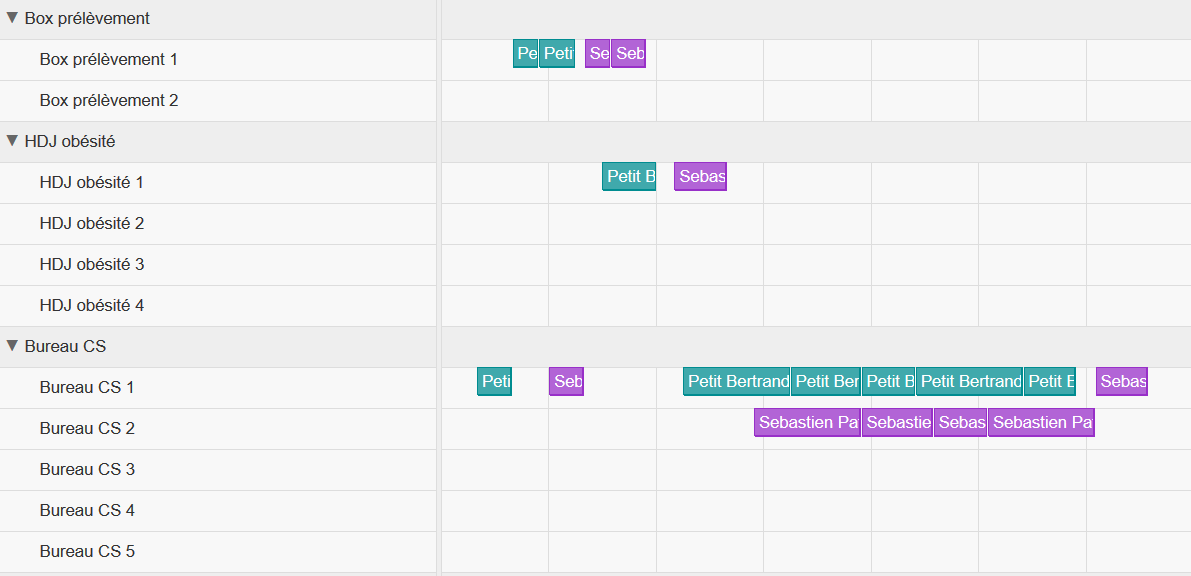
\includegraphics[scale=0.27]{images/exemple_calendrier2}
\end{center}

\end{frame}


\section{Qualité de code}

\begin{frame}
\frametitle{SonarQube}

\begin{figure}
	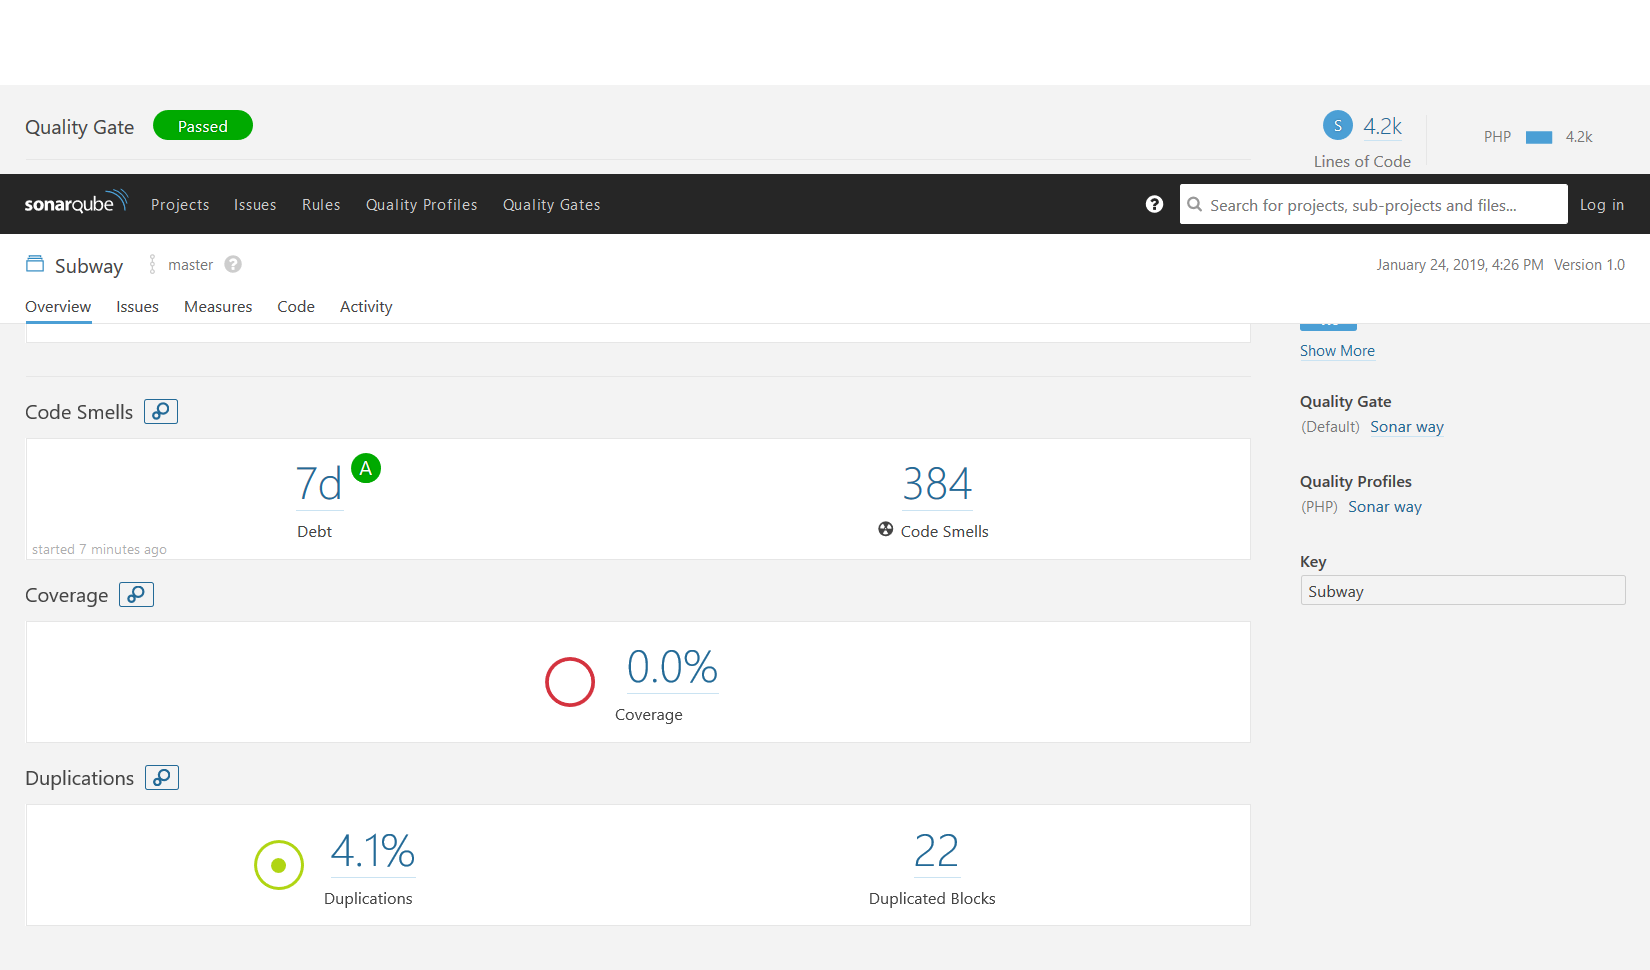
\includegraphics[scale=0.2]{images/sonar_scanner1}
\end{figure}

\end{frame}

\section{Tests}

\begin{frame}
\frametitle{Codeception}

Les tests ont été réalisés avec le framework \textit{Codeception}.

\bigbreak

Framework de tests de PHP:

\begin{itemize}
	\item Tests d'acceptances
	\item Tests fonctionnels
	\item Tests unitaires (basé sur PHPUnit)
\end{itemize}

\end{frame}

\begin{frame}
\frametitle{Tests pour la planification}

Tests des différents cas possibles de planification

\bigbreak

\begin{itemize}
	\item Planification avec un patient
	\item Tests de planification pour chaque parcours
	\item Planification avec plusieurs patients
\end{itemize}

\bigbreak

Certains cas restent à corriger (par exemple, planification avec une activité déjà placée sur le calendrier)


\end{frame}


\section*{Conclusion}

\begin{frame}
\frametitle{Améliorations à faire}

Ils restent de nombreuses améliorations possibles sur l'outil:

\bigbreak

\begin{itemize}
	\item Étoffer la planification pour ajouter des options (démarrer au plus tôt, minimiser le temps d'attente, ...)
	\item Ajouter la création de jeux de données automatisée pour les tests
	\item Implémentation de la planification en temps réel
	\item et d'autres encore...
\end{itemize}

\end{frame}

\begin{frame}
\frametitle{Bilan personnel}

Ce projet m'a apporté des compétences techniques (nouveaux langages et framework) mais aussi en terme d'analyse et d'évolutivité.

\bigbreak

Disponible sur \textbf{GitHub} à l'adresse \url{https://github.com/RomainR37/ParcoursPatient}

\end{frame}

\end{document}